\documentclass[12pt]{article}
\usepackage[margin=1.2in]{geometry}
\usepackage{amsmath}
\usepackage{graphicx}
\usepackage{caption}
\usepackage{amssymb}
\usepackage{subcaption}
\usepackage{multirow}
\usepackage{makecell}
\usepackage{tabu}
%\renewcommand{\labelitemii}{$\circ$}
\begin{document}
\title{COL334 - Assignment 2\\ HTTP}
\author{Akshay Kumar Gupta\\\texttt{2013CS50275} \and  Barun Patra\\\texttt{2013CS10773} \and Haroun Habeeb\\\texttt{2013CS10225}}
\date{}
\maketitle
\noindent 
We ran our python scripts ( Q4.py, timing.py ) on the two Object Tree files, namely, www.nytimes.com.objt and www.vox.com.objt. All data collection was performed on the same network, i.e, Airtel Broadband.
\\\\\\
{\bfseries Q4a. Overview} %TODO : Brief overview of code?
\\\\\texttt{Q4.py:} The script takes in as input an \texttt{Object Tree} or a \texttt{HAR file}, the \texttt{maximum allowed TCP connections} per domain, and the \texttt{maximum number of objects} per TCP connection. If the input is a \texttt{HAR file}, it is first converted to an \texttt{Object Tree} and then processed. \\
Each layer of the \texttt{Object Tree} is processed sequentially, i.e objects of parents are downloaded before the objects of the children. At every layer, objects belonging to a domain are passed to the thread.\\
In the thread, at any given time, \texttt{TCP connections} $\leq$ \texttt{(TCP connections)$_{max}$} are opened in parallel to the domain in consideration, with each TCP connection requesting and downloading \texttt{objects} $\leq$ \texttt{(objects)$_{max}$}. Downloading across domains is done in parallel on separate threads.
\\\\
\texttt{timing.py} This script imports Q4.py and runs the downloader for all possible combinations of \texttt{tcp$_{max}$} and \texttt{obj$_{max}$} less than upper limits given by command line input.
~\\\\
\textbf{Problems Faced during implementation:}
\begin{itemize}
\item \textbf{HTTPS and HTTP on same domain}: This problem arises because some domains have objects that are requested by HTTP and some others by HTTPS. This ensures that we couldn't just use one type of socket per domain. If we were to use TCP Sockets connected to port 80, the HTTPS objects wouldn't download.\\
\textit{Solution}: The simple workaround is to treat HTTPS objects as being from a different domain entirely. Or, while sending the requests from a domain, once you have sent all the HTTP requests, open a socket to port 443 and send the HTTPS requests. We used python's inbuilt ssl API to create secure sockets.
\item \textbf{Tolerance in the Protocol} We noticed that a lot of domains, in their response, do not mention headers such as Content-Length, some of them even misspelt "Connection". Some of them respond with a "Connection: close" although our request contained a "Connection: keep-alive". Some domains just timed out, causing our thread to break.
\\\textit{Solution:} Redundancy solves most of these issues. i.e, in case a certain request fails, we resend all the requests after that request.
\item \textbf{Network Conditions}: To appropriately measure the data required in later parts, we needed to replicate the network conditions. This was a problem we identified early on. The fact that running it for a wide range of parameters takes at least 30 minutes meant that network conditions would change while our program was still running. 
\textit{Solution:} We collected data late in the night, post midnight. This solution doesn't account for international network conditions changing.
\end{itemize}
%%%%%%%%%%%%%%%%%%%
%%%%%%%%%%%%%%%%%%%
{\bfseries Q4c.}
\\The parameters obtained from Q3c. were \texttt{tcp$_{max}$} = 6 and \texttt{obj$_{max}$} = 4
\begin{itemize}
\item \textbf{nytimes}: 
\begin{itemize}
	\item TCP Connections: 6
	\item Number of Objects: 4
	\item Browser Time: 68s
	\item Downloader Time: 15.20
\item The large browser time could be explained by the fact that some requests such that as those from ping.chartbeat.net happen only long after the rest of the webpage has been loaded. However, in the downloader, these requests are done in parallel with the rest of the webpage.
\end{itemize}

\item \textbf{vox}:
\begin{itemize}
	\item TCP Connections: 6
	\item Number of Objects: 4
	\item Browser Time: 53s
	\item Downloader Time: 123.77
	\item On a different day, we did manage to get about 55s for the downloader time, however, that data had a very large number of outliers because others were using the same internet connection.
\end{itemize}
\end{itemize}
We fail to reach any conclusion from just this data. However, the reason for abnormality have been mentioned.
~\\\\\\
{\bfseries Q4d. Running time for different parameters}
\\\\
Following is a tabular form our observations.\\
There are quite a few discrepancies, and they are more pronounced for nytimes because of the smaller page load times. This in itself shows the massive dependence on network conditions. 
\\\\
\hspace*{-1cm}
\begin{tabu} to 17cm { | X[c] | X[c] | X[c] | X[c] | X[c] | X[c] | X[c] | X[c] | X[c] |}
\hline
\hspace*{0.4cm}TCP  & \multirow{2}{}{1} & \multirow{2}{}{2} & \multirow{2}{}{3} & \multirow{2}{}{4} & \multirow{2}{}{5} & \multirow{2}{}{6} & \multirow{2}{}{7} & \multirow{2}{}{\hspace*{-0.7cm}Average}\\
\hspace*{-0.4cm}OBJ & & & & & & & & \\
\hline 
1 & 16.875 & 66.887 & 14.677 & 10.637 & 33.861 & 14.829 & 24.142 & 25.987 \\
\hline
2 & 13.312 & 11.892 & 12.064 & 11.032 & 15.001 & 10.343 & 13.65 & 12.471 \\
\hline
3 & 11.188 & 13.61 & 13.094 & 16.674 & 13.579 & 13.313 & 16.766 & 14.032 \\
\hline
4 & 16.858 & 13.531 & 13.266 & 11.828 & 66.654 & 15.204 & 13.881 & 21.603 \\
\hline
5 & 11.713 & 15.485 & 64.456 & 13.923 & 13.329 & 13.235 & 15.905 & 21.149 \\
\hline
6 & 13.08 & 11.132 & 12.688 & 14.172 & 11.743 & 17.001 & 66.348 & 20.881 \\
\hline
7 & 13.594 & 65.455 & 29.345 & 16.71 & \textbf{9.907} & 25.439 & 11.391 & 24.549 \\
\hline
Average & 13.803 & 28.285 & 22.799 & 13.568 & 23.439 & 15.623 & 23.155 & 20.096 \\
\hline
\end{tabu}
~\begin{center}Table 1: Time taken (in seconds) for combinations of parameters, nytimes \end{center}
~\\\\
\hspace*{-1cm}
\begin{tabu} to 17cm { | X[c] | X[c] | X[c] | X[c] | X[c] | X[c] | X[c] | X[c] | X[c] |}
\hline
\hspace*{0.4cm}TCP  & \multirow{2}{}{1} & \multirow{2}{}{2} & \multirow{2}{}{3} & \multirow{2}{}{4} & \multirow{2}{}{5} & \multirow{2}{}{\textbf{6}} & \multirow{2}{}{\textbf{7}} & \multirow{2}{}{\hspace*{-0.7cm}Average}\\
\hspace*{-0.4cm}OBJ & & & & & & & & \\
\hline 
1 & 153.35 & 131.99 & 127.92 & 147.40 & 139.24 & 120.91 & 125.58 & 135.20 \\
\hline
2 & 136.49 & 139.90 & 126.65 & 124.11 & 127.43 & 124.09 & 135.62 & 130.61 \\
\hline
3 & 133.67 & 130.81 & 124.80 & 120.46 & 125.79 & 125.02 & 121.30 & 125.98 \\
\hline
4 & 133.49 & 125.32 & 122.99 & 121.86 & 123.56 & 123.78 & 121.94 & 124.71 \\
\hline
\textbf{5} & 131.57 & 130.74 & 121.64 & 121.47 & 123.75 & \textbf{119.68} & 119.81 & 124.10 \\
\hline
6 & 129.58 & 145.27 & 125.94 & 124.21 & 123.09 & 120.67 & 122.27 & 127.29 \\
\hline
7 & 189.62 & 128.58 & 122.15 & 126.92 & 125.74 & 124.62 & 123.50 & 134.45 \\
\hline
Average & 129.58 & 133.23 & 124.59 & 126.63 & 126.94 & 122.68 & 124.29 & 128.38 \\
\hline
\end{tabu}
~\begin{center}Table 2: Time taken (in seconds) for combinations of parameters, vox \end{center}
~\\
%%%%%%%%% End of tables
\begin{center}
\emph{The minima have been shown in bold in the table.}\\\\
\end{center}
%%%%%%%%% Beginning of charts
\hspace*{0.6cm}
{\centering{
{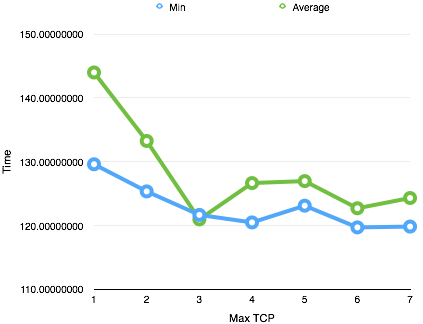
\includegraphics[scale=0.8]{Charts/vox_superpose.png}
}
}
}
%\vspace*{-0.6cm}
\begin{center}Figure 1: Time taken to download vox, min time and average time (over number of objects) plotted against number of tcp connections\end{center}

\hspace*{0.6cm}
{\centering{
{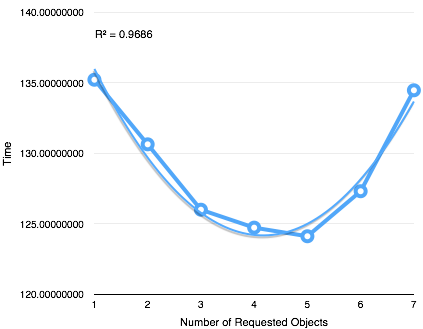
\includegraphics[scale=0.8]{Charts/vox_avg_over_tcp.png}
}
}
}
%\vspace*{-0.6cm}
\begin{center}Figure 2: Time taken to download vox, averaged over max. number of tcp connections\end{center}

\hspace*{0.6cm}
{\centering{
{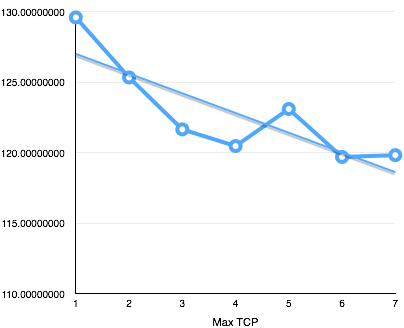
\includegraphics[scale=0.8]{Charts/vox_avg_over_obj.png}
}
}
}
%\vspace*{-0.6cm}
\begin{center}Figure 3: Time taken to download vox, averaged over max. number of objects\end{center}

\hspace*{0.6cm}
{\centering{
{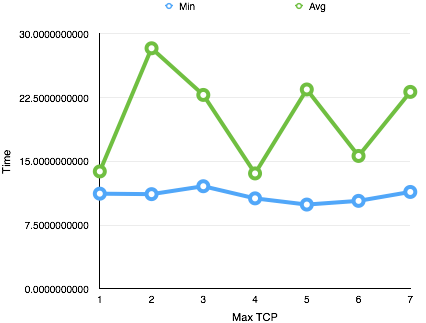
\includegraphics[scale=0.8]{Charts/nytimes_superpose.png}
}
}
}
%\vspace*{-0.6cm}
\begin{center}Figure 4: Time taken to download nytimes, min time and average time (over number of objects) plotted against number of tcp connections\end{center}

\hspace*{0.6cm}
{\centering{
{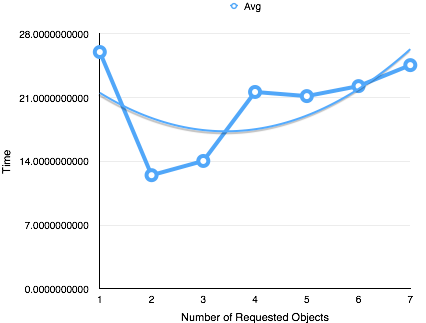
\includegraphics[scale=0.8]{Charts/nytimes_avg_over_tcp.png}
}
}
}
%\vspace*{-0.6cm}
\begin{center}Figure 5: Time taken to download nytimes, averaged over max. number of tcp connections\end{center}

\hspace*{0.6cm}
{\centering{
{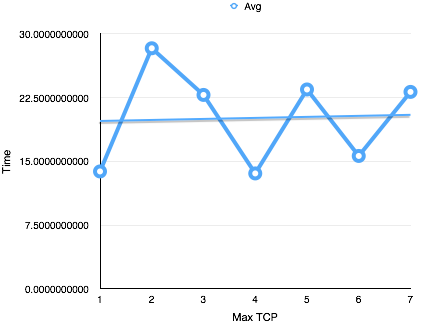
\includegraphics[scale=0.8]{Charts/nytimes_avg_over_obj.png}
}
}
}
%\vspace*{-0.6cm}
\begin{center}Figure 6: Time taken to download nytimes, averaged over max. number of objects\end{center}


\begin{itemize}
\item \textbf{Discrepancies}\\
\begin{itemize}
\item \textit{Existance}: From the graphs, it is obvious that discrepancies do exist. These discrepancies are more pronounced for nytimes because it takes a smaller amount of time to download. These discrepancies are largely due to network conditions. 
\item \textit{Minimization}: To minimize them, we ran our scripts late in the night ( between 12am and 3am ) when congestion is expected to be less. However, the discrepancies do still exist, and we will have to manage with them. 
\item \textit{Impact}: The impact on nytimes is fairly large and obvious, while for vox, the impact is less pronounced. Infact, the impact on nytimes is enough to outweigh the effect of increasing TCP as shown by Figure 6. For example, there are download times of 9s and also download times of 60s.
\end{itemize}
Hence, we can say that for smaller websites, the network conditions matter more than our choice of parameters. However, for larger websites, the discrepancies are less pronounced and hence the parameters do matter.
%%%%%%%%%%%%
\item \textbf{Average Time $_{over tcp}$ vs Max. objects}:\\ Referring to Figure 2 and Figure 5, we see that the time first decreases and then increased. The increase can be associated with the way we allocate objects to sockets.
\\ \textit{Reason}: Two factors that might be behin this trend are as follows : \begin{itemize}
\item Overhead: As the max.obj decreases, the downloader needs to create more TCP Connections. This creates more overhead. Hence, as max. obj increases, the amount of overhead decreases.
\item Task Management : We followed a greedy approach to allocate objects to sockets. For example, if we can have 4 threads, and have max.obj = 3 and have 4 objects remaining, we allot the first thread 3 objects and then 1 to the second. Within this example, if we were to increase max.obj to 5, the new allotment would be 4 objects to the first thread, and 0 to the rest. Hence, the time taken would increase as max.obj increase. 
\end{itemize}
The above two reasons gave rise to a graph that first decreases then increases. Hence, a "sweet spot" exists for our choice of number of max.obj
%%%%%%%%%%%%
\item \textbf{Average Time $_{over obj}$ vs Max. TCP Connections}\\
Referring to Figures 3 and 6. If we were to consider nytimes and vox, we would not be able to reach a conclusion. However, since we can ignore nytimes ( network dependence ), we will now proceed to reach a conclusion from Figure 3. We will also consult Figure 1 which plots the min. time over max. obj plotted against max. TCP Connections.
\begin{itemize}
\item \textit{Observation} There is a clear downward trend. i.e., As we increase the number of TCP Connections allowed, the time taken reduces.
\item \textit{Reason} The reason behind this is quite simply put parallelism. It was expected as long as the network dependence wasn't too high. However, we don't expect this to extrapolate to infinity because the server load would certainly increase. We believe the graph might flatten out as the benefit of adding another TCP Connection reduces as we increase the number of TCP Connections.
\item \textit{Conclusion} Increasing the number of TCP Connections until a reasonable number will certainly help us.
\end{itemize}
\item \textbf{Expected Minima} From the above two trends, we'd expect the optimal parameters to be around \texttt{tcp}$_{max}$ = 7 and \texttt{obj}$_{max}$ = 4.
\begin{itemize}
\item nytimes: \texttt{tcp}$_{max}$ = 5 and \texttt{obj}$_{max}$ = 7
\\ \begin{itemize}
\item The time taken for these parameters is not too far off from the time taken for \texttt{tcp}$_{max}$ = 7 and \texttt{obj}$_{max}$ = 4
\end{itemize}
\item vox : \texttt{tcp}$_{max}$ = 6 and \texttt{obj}$_{max}$ = 5
\\ \begin{itemize}
\item The time taken for (6,4) is 119.68s while the time taken for (7,4) is 121.94s . We can conclude that our analysis holds for vox.
\end{itemize}
\end{itemize}

%%%%%%%%%%%%
\end{itemize}
~\\\\
%%%%%%%%%
{\bfseries Q4e. Improving Running Time: }
\\ Some points of improvement are as follows:
\begin{itemize}
\item \textbf{Managing Data Distribution:} In the implemented downloader, objects belonging to the same domain are distributed to different threads, taking into consideration the maximum objects a connection can handle at any given time. A better way to carry out this distribution would be to ensure every TCP connection gets (more or less) an even split in terms of the size of data being downloaded on the same, to ensure maximum benefit of parallelization. The file sizes can be taken from the HAR file. As for the HTTP/HTML standards, incase each reference comes with the content size, this strategy can be implemented for a browser, i.e, if a html page contains an image, if it saves the size of the image along with the location, the aforementioned strategy can be implemented.
\item \textbf{Scheduling of Threads:} In the implemented version of the downloader, for a given domain, at most $K$ ($K$ $=$ \texttt{(TCP connections)$_{max}$}) threads are spawned, each establishing its own TCP connection. Then, the downloader waits for all the threads to join, before continuing, in order to ensure that at most $K$ connections are opened at any given time to the server. This can be improved by not waiting for the thread join. Instead, at the end of each thread execution, another thread can be spawned then to handle the next batch of requests. This can be used, in conjunction with the aforementioned improvement to ensure the newly spawned thread takes up an optimal number of objects instead of the maximum allowed number of objects, so as to, again, maximize the benefits of parallelization.  
\item \textbf{Number of TCP connections opened to a domain:} The HAR file can be used to infer the maximum number of TCP connections that a server allows in parallel(i.e if the server places a cap on the maximum allowed connections). Using this information, we can dynamically allocate the value of $K$ for different domains for the case of large files; so that the overhead of creating new threads and making a new TCP connection does not outweigh the benefit of parallization. 
\item \textbf{Congestion Sensitivity:} Since the network conditions matter a lot for page load times, it only makes sense to exploit the congestion data if possible. A simple way to do this would be to measure the RTT of each connection and then allocate objects for download depending on the RTT. Hence, if one of our sockets uses a path with higher congestion, we would download less data on it.
\item \textbf{Fractional Requests:} In the case that the server sets a cap on the bandwidth allocated to a single TCP connection, large objects can be requested in chunks on separate TCP connections, with each TCP connection requesting for a fraction of the file.
\end{itemize}

\end{document}